\documentclass[a4paper]{article}
\usepackage[utf8]{inputenc} % accents xuten bé
\usepackage[T1]{fontenc} % també pels accents, meh
\usepackage[catalan]{babel} % idioma
\usepackage{titlesec} % per a canviar format dels títols
\usepackage{titling} % per a poder definir \subtitle
%\usepackage[none]{hyphenat} % no separa paraules
\usepackage{mathtools} % millor que amsmath (opcions de notació mates)
\usepackage{amsfonts} % segurament per definir = amb coses dalt
\usepackage{cases} % per poder fer les típiques definicions per parts de funcions amb corxets
\usepackage{blindtext} % textos de prova, tipus loremipsum
\usepackage{enumitem} % llistes
\usepackage{geometry} % per controlar els marges
\usepackage{indentfirst} % per controlar la indentació de la primera línia de cada paràgraf
\usepackage{physics} % sobretot, derivades (parcials)
\usepackage{xcolor} % colors
\usepackage{float} % per controlar posicions de flotants (imatges i taules)
\usepackage{hyperref}
\usepackage{multirow}
\usepackage[per-mode=symbol]{siunitx}
\usepackage{graphicx}
\usepackage{caption}
\usepackage{subcaption}
%\usepackage{biblatex}
%\usepackage[
%backend=biber,
%style=alphabetic,
%citestyle=authoryear
%]{biblatex}

\usepackage{graphicx} % alguna cosa per a imatges
\graphicspath{ {./images/} }

% Que la primera línia no estigui indentada
\setlength{\parskip}{\baselineskip}
\setlength{\parindent}{0cm}

%\titlelabel{\llap{\thetitle\quad}} % No indentació dels títols

%Marges
%\hoffset = 0in
%\oddsidemargin = 13pt
%\textwidth = 427pt

%Comandes útils
\newcommand\eqdef{\mathrel{\overset{\makebox[0pt]{\mbox{\normalfont\tiny\sffamily def}}}{=}}}
\newcommand\eqimp{\mathrel{\overset{\makebox[0pt]{\mbox{\normalfont\tiny\sffamily imp}}}{=}}}
\newcommand\eqtext[1]{\mathrel{\overset{\makebox[0pt]{\mbox{\normalfont\tiny\sffamily {#1}}}}{=}}}
\renewcommand\vnabla{\vec{\nabla}}
\newcommand\vecv{\vec{v}}
\newcommand{\vvec}[1]{\vec{\vec{#1}}}
\newcommand\vecdot[1]{\dot{\vec{#1}}}
\newcommand\redtext[1]{\textcolor{red}{#1}}
\newcommand{\ten}[2]{\ensuremath{{#1}\times 10^{#2}}}
\DeclareMathOperator\arctanh{arctanh}

% definició de \subtitle
\newcommand{\subtitle}[1]{%
  \posttitle{%
    \par\end{center}
    \begin{center}\large#1\end{center}
    \vskip0.5em}%
}

% Format dels títols
\titleformat*{\section}{\Large\bfseries}
\titleformat*{\subsection}{\bfseries}

\captionsetup{
    width=\textwidth, % width of caption is 90% of current textwidth
    labelfont=bf,        % the label, e.g. figure 12, is bold
    font=small,          % the whole caption text (label + content) is small
%    format=hang,         % no caption text under the label
}

% Si funcionés, algun format de pàgina
%\pagestyle{fancy}
%\fancyhf{}
%\rhead{Share\LaTeX}
%\lhead{Guides and tutorials}
%\rfoot{Page \thepage}

% AND HERE WE GO

\title{\textbf{Simulació 2D del Model d'Ising}}
\subtitle{\scshape{Fenòmens col·lectius i transicions de fase}}
\author{Ivan Alsina Ferrer}
\date{}

\begin{document}

\maketitle

\section{Introducció}

El model d'Ising té una importància cabdal en física estadística perquè proporciona una sèrie de tècniques matemàtiques per a treballar amb xarxes $n$-dimensionals de partícules que permeten entendre el comportament crític d'una gran varietat de sistemes a la natura. L'hamiltonià que proporciona és el següent:
\begin{equation*} \label{ising_hamiltonian}
    \mathcal{H}^* \equiv \mathcal{H}/J = -\sum_\text{nn} \sigma_i \sigma_j - \frac{B}{J} \sum_{i=1}^{N} \sigma_i
\end{equation*}
on $\mathcal{H}^*$ és l'hamiltonià reduït, és a dir, en unitats de l'energia d'interacció entre les partícules $J$. nn fa referència a \textit{nearest neighbors}, o \textit{primers veïns}, indicant que el sumatori involucrat s'exten sobre les parelles de partícules que estan a distància mínima. $B$ és el camp aplicat, en unitats de $\mu$, però en el nostre cas no en considerarem el terme ja que l'estudi ha estat considerant camp nul.

El treball que presentem estudia un sistema bidimensional de $N$ partícules, distribuïdes segons una matriu $L\times L$, i descrites per un spin, representat com a $\sigma_i$ en l'equació \eqref{ising_hamiltonian}. Aquest pot estar orientat en dues direccions: bé amunt (valor $+1$) o avall (valor $-1$). L'estat fonamental d'aquest sistema, quan es troba a una temperatura fixada, minimitza l'energia lliure de Helmholtz.
\begin{equation*}
    F = U - TS
\end{equation*}
Per a fer-ho, pot minimitzar l'energia interna $U$ o bé maximitzar l'entropia $S$. Un sistema a baixa temperatura mostra el primer comportament, i es diu que està en la seva fase ordenada. Un sistema a alta temperatura, en canvi, té preferència pel segon, mostrant-se en la seva fase desordenada. El pas d'un comportament a l'altre constitueix una transició de fase i és el que estudiarem amb detall en el present treball tot descrivint amb detall el comportament de les propietats termodinàmiques prop de la temperatura a què això té lloc, la temperatura de Curie ($T_c$).

Per a dur aquest estudi a terme, havent partit d'una configuració aleatòria d'spins, hem emprat l'algorisme de Metròpolis amb què, valent-se d'un gran nombre d'iteracions Montencarlo, s'han explorat les cadenes de Markov que descriuen el sistema. En cadascuna d'aquestes iteracions, s'han fet $N$ propostes de canvi d'spin, de manera aleatòria. Les propostes que suposen una disminució de l'energia s'accepten, i aquelles, en canvi que, suposen un augment de la mateixa, s'accepten amb probabilitat $\exp\left(-\Delta E^*/T^*\right)$. Això es tradueix en una penalització als canvis en spin que augmenten l'energia del sistema si l'increment es gran o si la temperatura a què es donen és baixa.

Ha estat necessari repetir el procés per a un gran nombre de llavors (que al cap i a la fi, és la component determinista de la simulació) per tal d'explorar amb comoditat tot l'espai de configuracions. Duent el compte de les energies i les imantacions s'han fet les mitjanes amb què després s'han trobat les propietats termodinàmiques d'interès. El procés s'ha repetit per a valors de temperatura reduïda en un rang de 1.5 a 3.5, i per a sistemes de longitud $L=15,30,45,60,75,90,120$.

\section{Evolució de imantacions i temperatures}

L'algorisme de Metropolis accepta els canvis en la configuració que comporten una variació d'energia negativa, i n'accepta aquells que comporten una variació d'energia positiva amb una probabilitat que decau exponencialment amb el valor d'aquesta variació, amb la qual cosa s'ajusta a la naturalesa probabilística de les fluctuacions en el sistema. És per aquest motiu que, tot i no haver definit una dinàmica pròpia del sistema, podem argumentar que les iteracions Montecarlo en la simulació donen una noció de l'evolució temporal d'un sistema que, partint d'una configuració inicial aleatòria (en el nostre cas, determinada per la seed que fem servir), es veuen sotmesos a una temperatura donada.


\begin{figure}[H]
    \centering
    \begin{subfigure}{.8\textwidth}
        \centering
        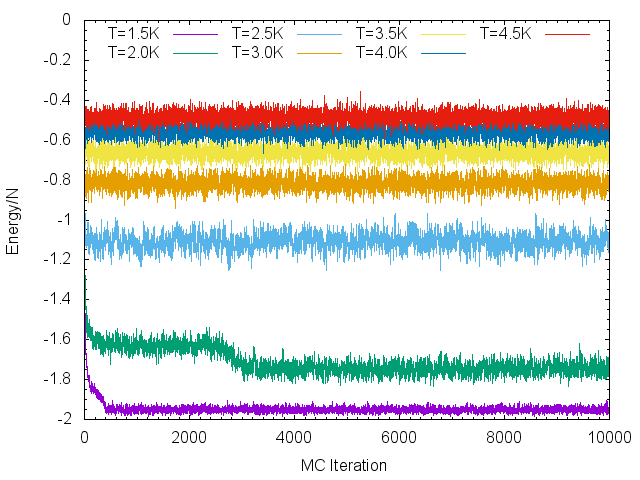
\includegraphics[width=0.8\textwidth]{SIM-L-060-energy-EVO.png}
        \caption{Energies per partícula}
        \label{fig:evo_ene}
    \end{subfigure}
    \begin{subfigure}{.8\textwidth}
        \centering
        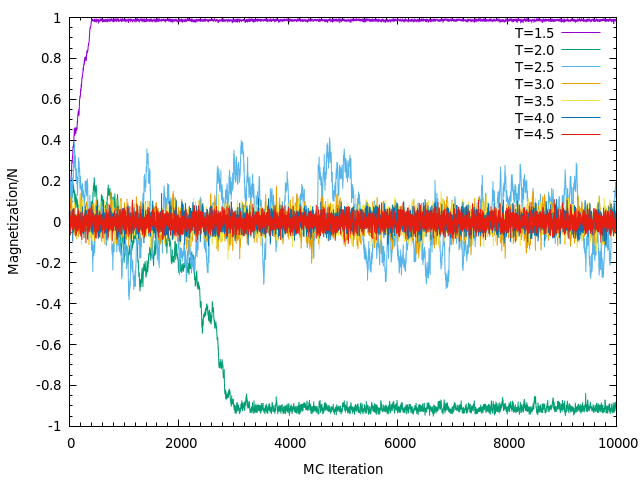
\includegraphics[width=0.8\textwidth]{SIM-L-060-magnetiz-EVO.png}
        \caption{Imantacions per partícula}
        \label{fig:evo_mag}
    \end{subfigure}
    \caption{Evolució de les energies per partícula i les imantacions per partícula al llarg de les iteracions Montecarlo, per a temperatures reduïdes $T^*$ en el rang 1.5 a 4.5, en un sistema quadrat de $L=60$ spins de costat.}
\label{fig:evo}
\end{figure}

Tal com veiem a la figura \ref{fig:evo_ene}, per a temperatures baixes l'energia per partícula del sistema convergeix ràpidament a 2 cops l'energia de lligam, la qual cosa és deguda a que, per a temperatures baixes, com que el sistema minimitza l'energia
\begin{equation*}
    E^*/N = \langle \mathcal{H} \rangle / N= -\sum_{\langle{i,j\rangle}} 1/N = -\frac{1}{2}z = -2
\end{equation*}
en què $z$ és el nombre de coordinació ($z=4$) i on recordem, treballem en unitats reduïdes d'energia: l'energia es troba dividida entre $J$, l'energia de lligam de partícula. A temperatures altes, en canvi, el sistema es troba en la fase desordenada i tendeix a maximitzar l'entropia. Això significa que, en promig, hi haurà molt poques partícules que tinguin veïnes orientades en el mateix sentit, provocant que l'energia per partícula sigui, en valor absolut, petita.

Quant a la imantació, representada a la figura \ref{fig:evo_mag}, observem com per a temperatures baixes convergeix ràpidament a 1 o -1, ja que totes les partícules tendeixen a alinear-se en la mateixa direcció. El signe ve determinat per la pròpia evolució del sistema que en principi és aleatòria, però en el nostre cas està governada pel generador de nombres aleatoris i la seed que triem. Així com augmentem la temperatura el sistema tendeix a mantenir la imantació propera a zero, pel mateix motiu que esmentàvem abans: llevat de fluctuacions, aproximadament la meitat dels spins estan orientats cap amunt, i l'altra, cap avall, cancel·lant així la imantació mitjana.

Així com augmentem les temperatures, es pot observar com hi ha una temperatura per la qual la imantació és altament fluctuant (en la figura \ref{fig:evo_mag}, $T*=2.5$). La raó és que aquesta temperatura és molt propera a la temperatura crítica del sistema i, tal com estudiarem més endavant, les correlacions es fan de molt llarg abast, de tal manera que l'estabilitat de les propietats termodinàmiques del sistema es veuen compromeses.

Presentem a continuació la configuració final del sistema després de 10 000 iteracions Montecarlo a temperatures alta i baixa, de forma que se'n posi de manifest la fase ordenada i desordenada, respectivament.

\begin{figure}[H]
    \centering
    \begin{subfigure}{.45\textwidth}
        \centering
        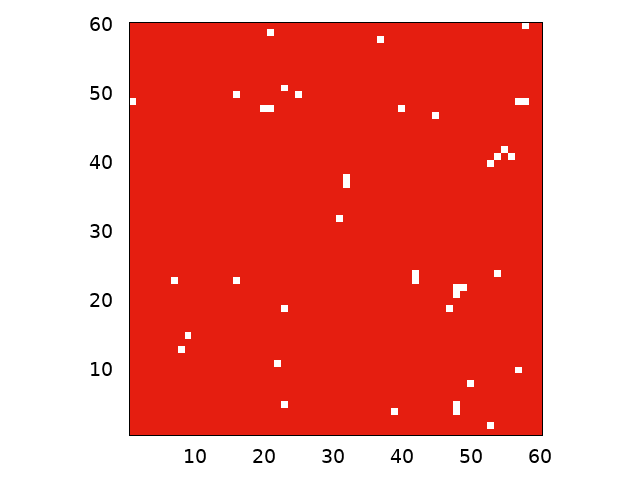
\includegraphics[width=\textwidth]{SIM-L-060-TEMP-1500.png}
        \caption{$T^*=1.5$}
        \label{fig:conf_low}
    \end{subfigure}
    \begin{subfigure}{.45\textwidth}
        \centering
        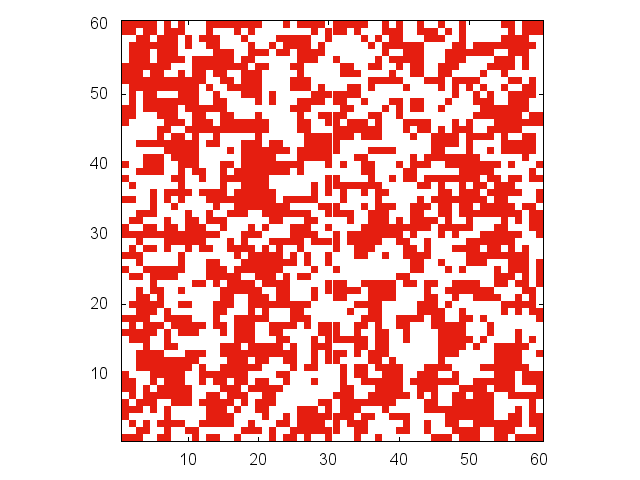
\includegraphics[width=\textwidth]{SIM-L-060-TEMP-4500.png}
        \caption{$T^*=4.5$}
        \label{fig:conf_high}
    \end{subfigure}
    \caption{Configuració final, després de 10 000 iteracions Montecarlo, del sistema amb $L=60$ spins de costat de què se'n mostrava l'evolució a la figura \ref{fig:evo}, per a les temperatures reduïdes $T^*=1.5$ i $T^*=4.5$. Els quadrats vermells representen spins orientats cap amunt. Els blancs, spins orientats cap avall.}
\label{fig:conf}
\end{figure}


\section{Magnituds termodinàmiques}

\begin{figure}[H]
    \centering
    \begin{subfigure}{.45\textwidth}
        \centering
        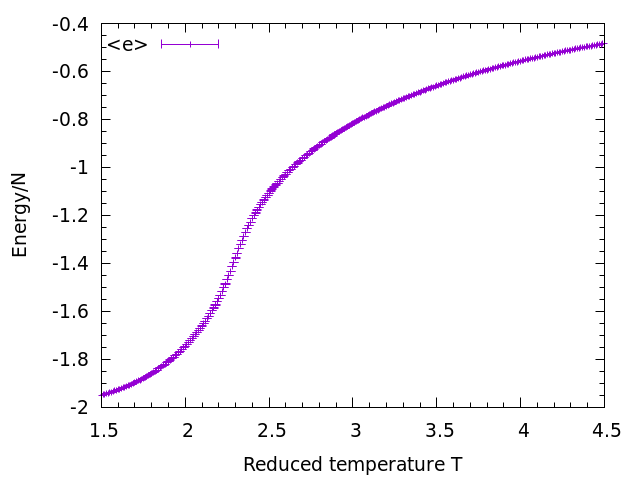
\includegraphics[width=\textwidth]{props-L-030_e.png}
        \caption{Energia per partícula}
        \label{fig:props-e}
    \end{subfigure}
    \begin{subfigure}{.45\textwidth}
        \centering
        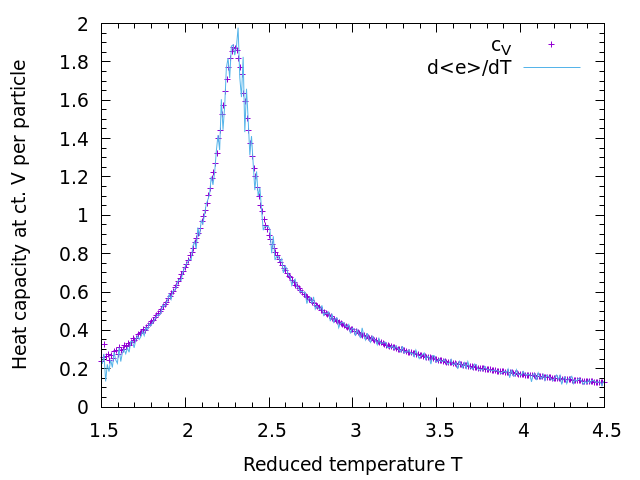
\includegraphics[width=\textwidth]{props-L-030_cvn.png}
        \caption{Capacitat calorífica per partícula}
        \label{fig:props-cv}
    \end{subfigure}
        \begin{subfigure}{.45\textwidth}
        \centering
        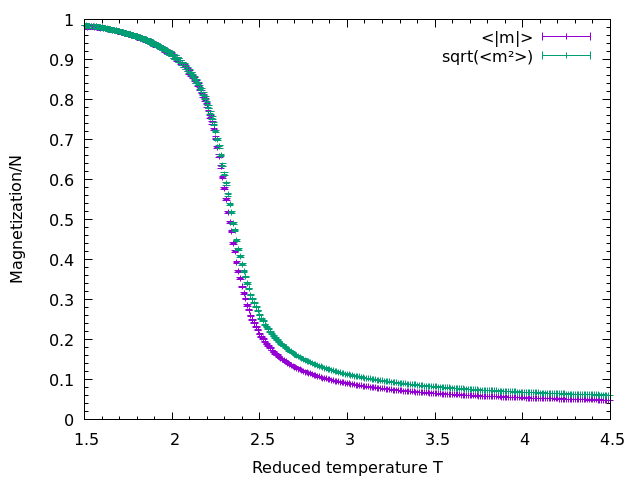
\includegraphics[width=\textwidth]{props-L-030_m.png}
        \caption{Imantació per partícula}
        \label{fig:props-m}
    \end{subfigure}
    \begin{subfigure}{.45\textwidth}
        \centering
        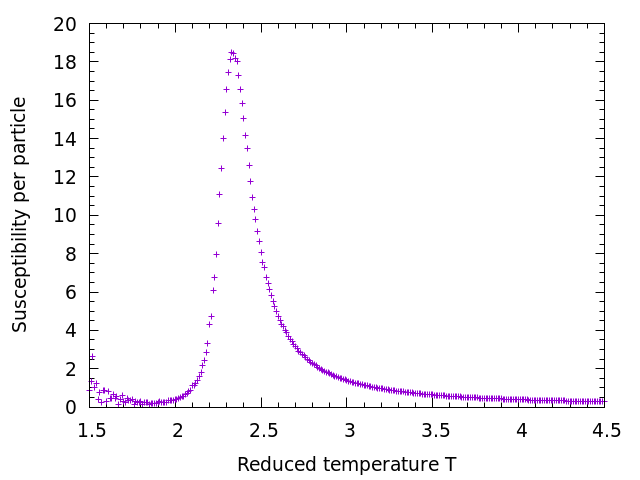
\includegraphics[width=\textwidth]{props-L-030_xn.png}
        \caption{Susceptibilitat per partícula}
        \label{fig:props-x}
    \end{subfigure}
    \caption{Resultats de la simulació per a $L=30$ d'energia, capacitat calorífica, imantació i susceptibilitat, totes les magnituds per partícula. La capacitat calorífica mostra es mostra calculada com la variança de l'energia entre el quadrat de la temperatura, i com a la derivada del valor esperat de l'eneria respecte de la temperatura.}
\label{fig:props}
\end{figure}

\section{Efecte de variar la mida}

\begin{figure}[H]
    \centering
    \begin{subfigure}{.45\textwidth}
        \centering
        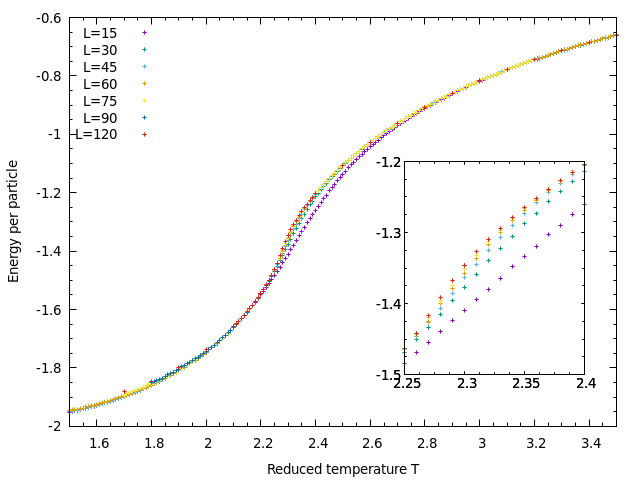
\includegraphics[width=\textwidth]{plot-e.png}
        \caption{Energia per partícula}
        \label{fig:plot-e}
    \end{subfigure}
    \begin{subfigure}{.45\textwidth}
        \centering
        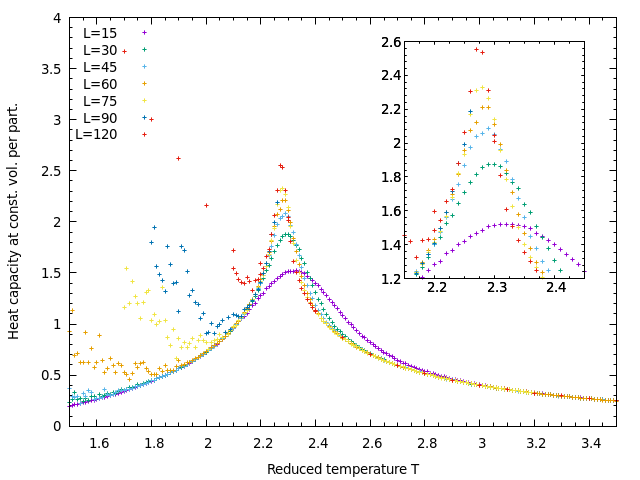
\includegraphics[width=\textwidth]{plot-cv.png}
        \caption{Capacitat calorífica per partíucla}
        \label{fig:plot-cv}
    \end{subfigure}
        \begin{subfigure}{.45\textwidth}
        \centering
        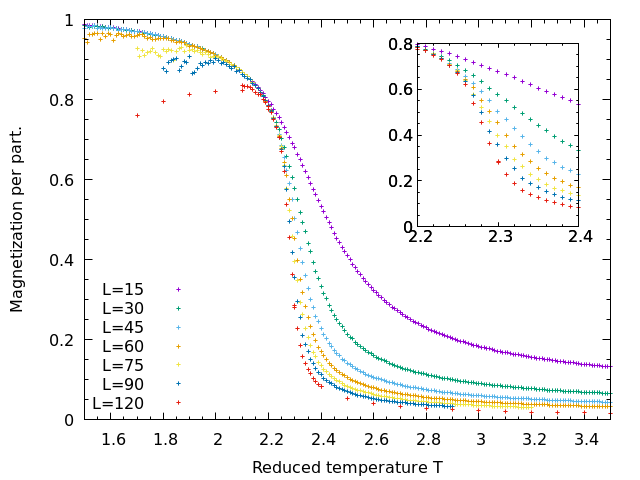
\includegraphics[width=\textwidth]{plot-m.png}
        \caption{Imantació per partícula}
        \label{fig:plot-m}
    \end{subfigure}
    \begin{subfigure}{.45\textwidth}
        \centering
        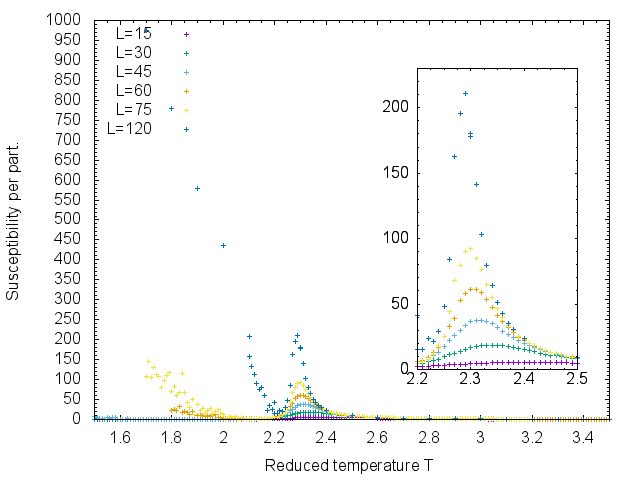
\includegraphics[width=\textwidth]{plot-x.png}
        \caption{Susceptibilitat per partícula}
        \label{fig:plot-x}
    \end{subfigure}
    \caption{Resultats de la simulació de la simulació per a l'energia, capacitat calorífica, imantació i susceptibilitat per a les diferents $L$, totes les magnituds per partícula. Es mostren les regions properes a la temperatura crítica ampliades.}
\label{fig:plot}
\end{figure}

\section{Temperatura crítica. Límit termodinàmic}

Trobar la temperatura crítica del model significa trobar la temperatura en què es dona la transició de fase en el límit termodinàmic, situació de $N \to \infty$, en què els efectes de les vores queden eliminats i el sistema és completament \textit{bulk}. Com que no podem simular un sistema amb $N$ infinita, estudiarem de manera quantitativa quina és la variació de la temperatura crítica amb $L$ per a cadascunes de les magnituds termodinàmiques estudiades, i n'extrapolarem el comportament a l'infinit.

Per a fer-ho, buscarem ajustos polinòmics als comportaments en les zones properes a $T_c$, d'ordre 3 en el cas de l'energia i la imantació, i d'ordre 2 en el cas de la capacitat calorífica i la susceptibilitat. D'aquesta forma, en podrem trobar numèricament els punt d'inflexió i els màxims, respectivament.

\begin{figure}[H]
    \centering
    \begin{subfigure}{.45\textwidth}
        \centering
        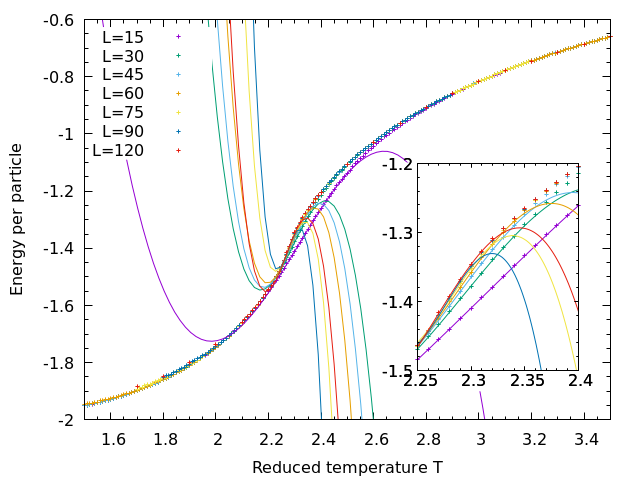
\includegraphics[width=\textwidth]{plot-e-fit.png}
        \caption{Energia per partícula}
        \label{fig:fit-e}
    \end{subfigure}
    \begin{subfigure}{.45\textwidth}
        \centering
        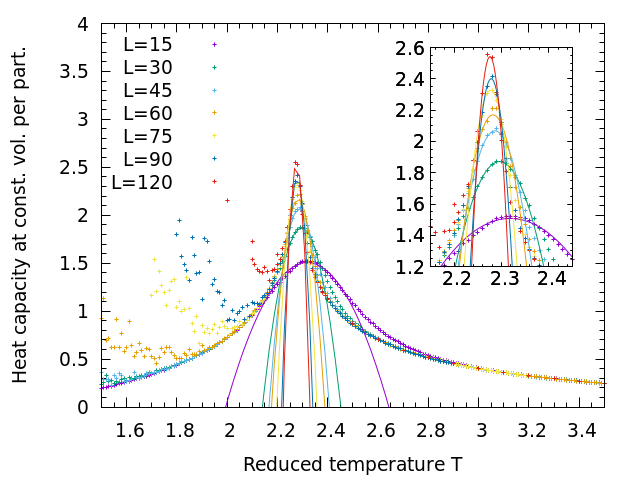
\includegraphics[width=\textwidth]{plot-cv-fit.png}
        \caption{Capacitat calorífica per partíucla}
        \label{fig:fit-cv}
    \end{subfigure}
        \begin{subfigure}{.45\textwidth}
        \centering
        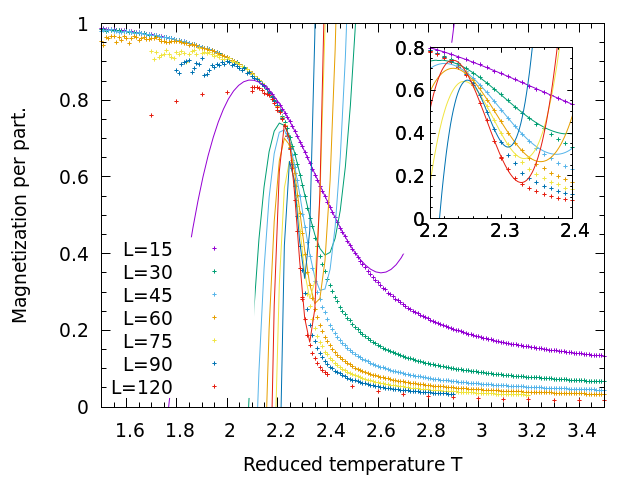
\includegraphics[width=\textwidth]{plot-m-fit.png}
        \caption{Imantació per partícula}
        \label{fig:fit-m}
    \end{subfigure}
    \begin{subfigure}{.45\textwidth}
        \centering
        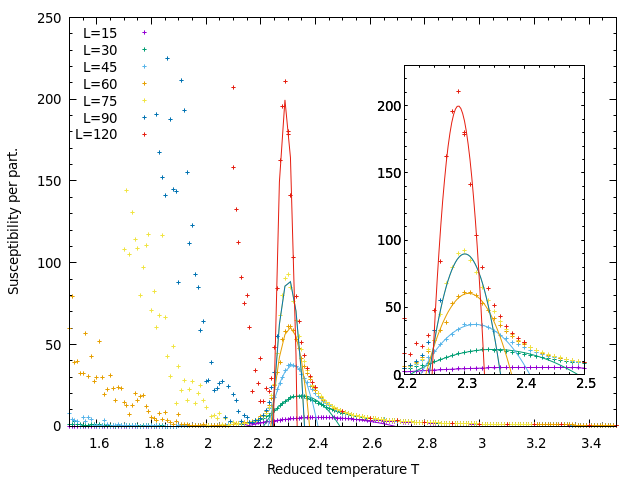
\includegraphics[width=\textwidth]{plot-x-fit.png}
        \caption{Susceptibilitat per partícula}
        \label{fig:fit-x}
    \end{subfigure}
    \caption{Figura \ref{fig:plot} a la qual s'hi han incorporat ajustos que descriuen les dades properes a la temperatura crítica: d'ordre 2 per a la capacitat calorífica i la susceptibilitat, i d'ordre 3 per a l'energia i la magnetització.}
\label{fig:fit}
\end{figure}

Un cop tenim aquests ajustos, podem representar els comportaments amb l'invers de la longitud de les temperatures crítiques d'energia i la imantació, segons el punt d'inflexió, i de la capacitat calorífica i la susceptibilitat, segons el màxim:

\begin{figure}[H]
    \centering
    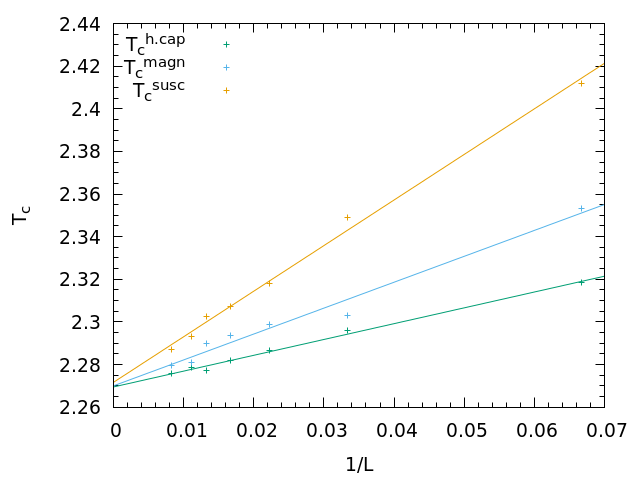
\includegraphics[width=.6\textwidth]{coefs-tc.png}
    \caption{Temperatures crítiques a $L$ finites. Es mostra la temperatura crítica contra $1/L$ i ajust lineal.}
    \label{fig:tc}
\end{figure}

Els ajustos de la figura \ref{fig:tc},
\begin{align*}
    T_c^{e} &= (6.64 \pm 0.09) + (2.270 \pm 0.003) \\
    T_c^{c_V} &= (0.74 \pm 0.02) + (2.2694 \pm 0.0008) \\
    T_c^{m} &= (1.22 \pm 0.09) + (2.270 \pm 0.003) \\
    T_c^{\chi} &= (2.14 \pm 0.07) + (2.271 \pm 0.002)
\end{align*}
tenen com a ordenada a l'origen la temperatura crítica que cadascuna de les magnituds termodinàmiques estudia.

Podem dir, doncs, que de manera conjunta, calculant-ne la mitjana i tenint en compte l'error estadístic:
\begin{equation}
    T_c = 2.2704 \pm 0.0009
\end{equation}
que està d'acord amb el valor teòric de la temperatura crítica:
\begin{equation}
    T_c^\text{teo} = \frac{2}{\ln(1+\sqrt{2})} \approx 2.2692
\end{equation}


\section{Exponents crítics}

\begin{figure}[H]
    \centering
    \begin{subfigure}{.45\textwidth}
        \centering
        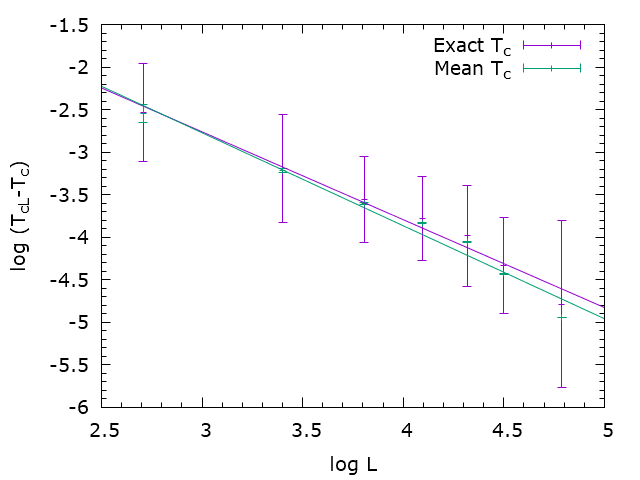
\includegraphics[width=\textwidth]{coefs-nu.png}
        \caption{Diferència de temperatures crítiques}
        \label{fig:coefs-nu}
    \end{subfigure}
    \begin{subfigure}{.45\textwidth}
        \centering
        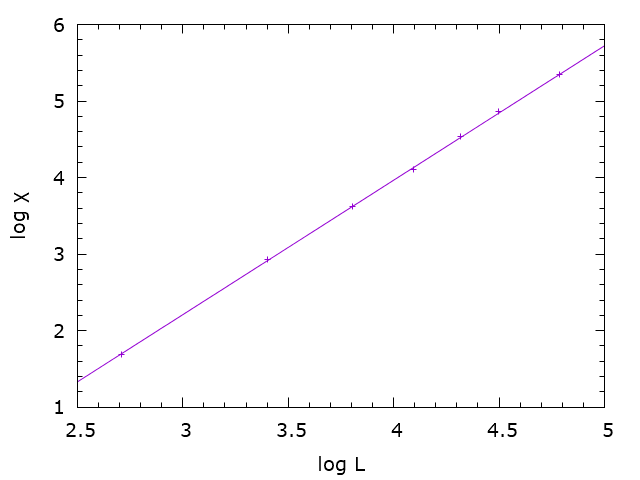
\includegraphics[width=\textwidth]{coefs-gammanu.png}
        \caption{Susceptibilitat}
        \label{fig:coefs-gammanu}
    \end{subfigure}
        \begin{subfigure}{.45\textwidth}
        \centering
        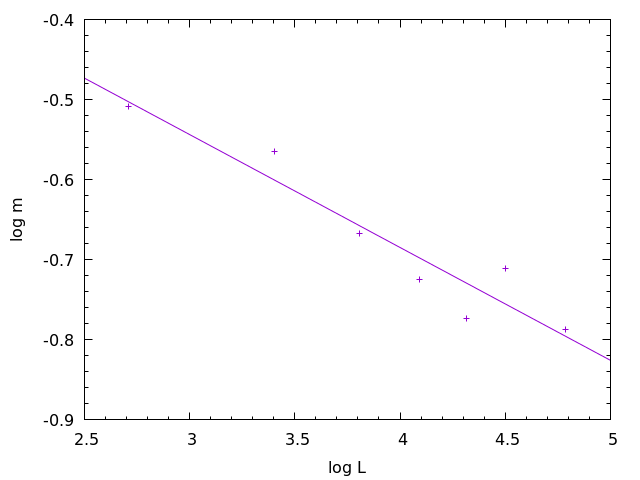
\includegraphics[width=\textwidth]{coefs-betanu.png}
        \caption{Imantació}
        \label{fig:coefs-betanu}
    \end{subfigure}
    \begin{subfigure}{.45\textwidth}
        \centering
        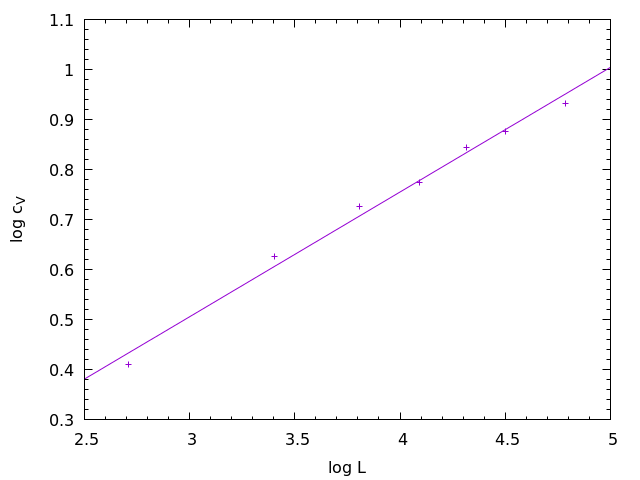
\includegraphics[width=\textwidth]{coefs-alphanu.png}
        \caption{Capacitat calorífica a volum constant}
        \label{fig:coefs-alphanu}
    \end{subfigure}
    \caption{Logaritme de les diferents magnituds termodinàmiques per partícula contra el logaritme de la longitud del costat de la matriu d'spins, amb els corresponents ajustos lineals. La figura \ref{fig:coefs-nu} mostra la diferència de la temperatura crítica en $L$ amb la temperatura crítica per un sistema infinit, calculada de manera exacta i segons la mitjana d'extrapolacions amb les diferents magnituds termodinàmiques.}
\label{fig:coefs}
\end{figure}

\begin{align*}
    \xi &= A \left| T-T_c \right|^{-\nu} = KL \\
    \left|T_{cL}-T_c \right| &= \left(\frac{K}{A} L \right)^{-1/\nu} \\
    \ln \left(T_{cL} - T_L \right) &= -\frac{1}{\nu} \ln L + \text{const}
\end{align*}

Si fem servir el valor exacte de la temperatura crítica del sistema:
\begin{equation*}
	T_c = \frac{2}{\ln \left(1+\sqrt{2} \right)}
\end{equation*}

\begin{equation*}
    \ln \left(T_{cL} - T_L \right) = (-1.03 \pm 0.07) \ln L + (0.3 \pm 0.3)
\end{equation*}

\begin{equation*}
	\nu = 0.97 \pm 0.06
\end{equation*}

\begin{equation*}
    \ln \left(T_{cL} - T_L \right) = (-1.09 \pm 0.08) \ln L + (0.5 \pm 0.3)
\end{equation*}

\begin{equation*}
	\nu = 0.91 \pm 0.07
\end{equation*}

\begin{align*}
	\chi &= C \left|T_{cL}-T_c\right|^{-\gamma} \\
	&= C \left[ \left(\frac{K}{A} L \right)^{-1/\nu} \right]^{-\gamma} \\
	&= C \left(\frac{K}{A} L \right)^{\frac{\gamma}{\nu}} \\
	\ln \chi &= \frac{\gamma}{\nu} \ln L + \text{const}
\end{align*}

\begin{equation*}
	\ln \chi_L = (1.757 \pm 0.010) \ln L + (-3.06 \pm 0.04)
\end{equation*}

\begin{equation*}
	\gamma = 1.70 \pm 0.12
\end{equation*}

\begin{equation*}
	\ln m_L = (-0.14 \pm 0.02) \ln L + (-0.12 \pm 0.08)
\end{equation*}

\begin{equation*}
	\beta = 0.136 \pm 0.010
\end{equation*}

\begin{equation*}
	\ln ({c_V})_L = (0.249 \pm 0.011) \ln L + (0.24 \pm 0.04)
\end{equation*}

\begin{equation*}
	\alpha = 0.24 \pm 0.03
\end{equation*}

\section{Finite size scaling}

\begin{figure}[H]
    \centering
    \begin{subfigure}{.45\textwidth}
        \centering
        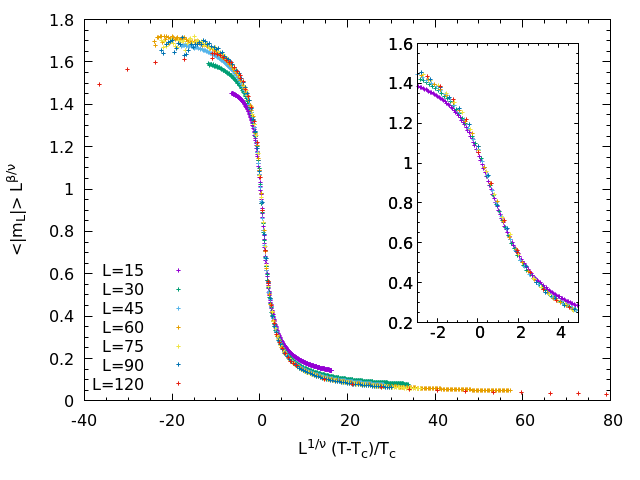
\includegraphics[width=\textwidth]{fss-m.png}
        \caption{}
        \label{fig:fss-m}
    \end{subfigure}
    \begin{subfigure}{.45\textwidth}
        \centering
        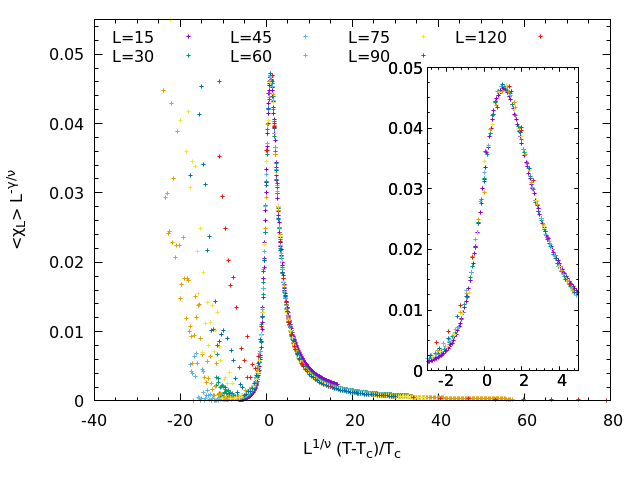
\includegraphics[width=\textwidth]{fss-x.png}
        \caption{}
        \label{fig:fss-x}
    \end{subfigure}
    \caption{Ey}
\label{fig:fss}
\end{figure}

\section{Conclusions}

\section{Referències}

\end{document}


